\section{TOPMODEL (model ID: 14)}
The TOPMODEL (fig.~\ref{fig:14_schematic}) is originally a semi-distributed model that relies on topographic information \citep{BEVEN1979}. 
The model(ling concept) has undergone many revisions and significant differences can be seen between various publications. 
The version presented here is mostly based on \citet{Beven1995}, with several necessary simplifications. 
Following \citet{Clark2008a}, the model is simplified to a lumped model (removing the distributed routing component) and all parameters are calibrated. 
This means the distribution of topographic index values that characterizes TOPMODEL are estimated using a shifted 2-parameter gamma distribution instead of being based on DEM data \citep{Sivapalan1987,Clark2008a}. 
For simplicity of the evaporation calculations, the root zone store and unsaturated zone store are combined into a single threshold store with identical functionality to the original 2-store concept. 
The model has 2 stores and 7 parameters ($S_{UZ,max}$, $S_t$, $K_d$, $q_0$, $f$, $\chi$, $\phi$). 
The model aims to represent:

\begin{itemizecompact}
\item Variable saturated area with direct runoff from the saturated part;
\item Infiltration and saturation excess flow;
\item Leakage to, and non-linear baseflow from, a deficit store.
\end{itemizecompact}

\subsection{MARRMoT model name}
m\_14\_topmodel\_7p\_2s \\

% Equations
\subsection{Model equations}

% Model layout figure
{ 																	% This ensures it doesn't warp text further down
\begin{wrapfigure}{l}{4cm}
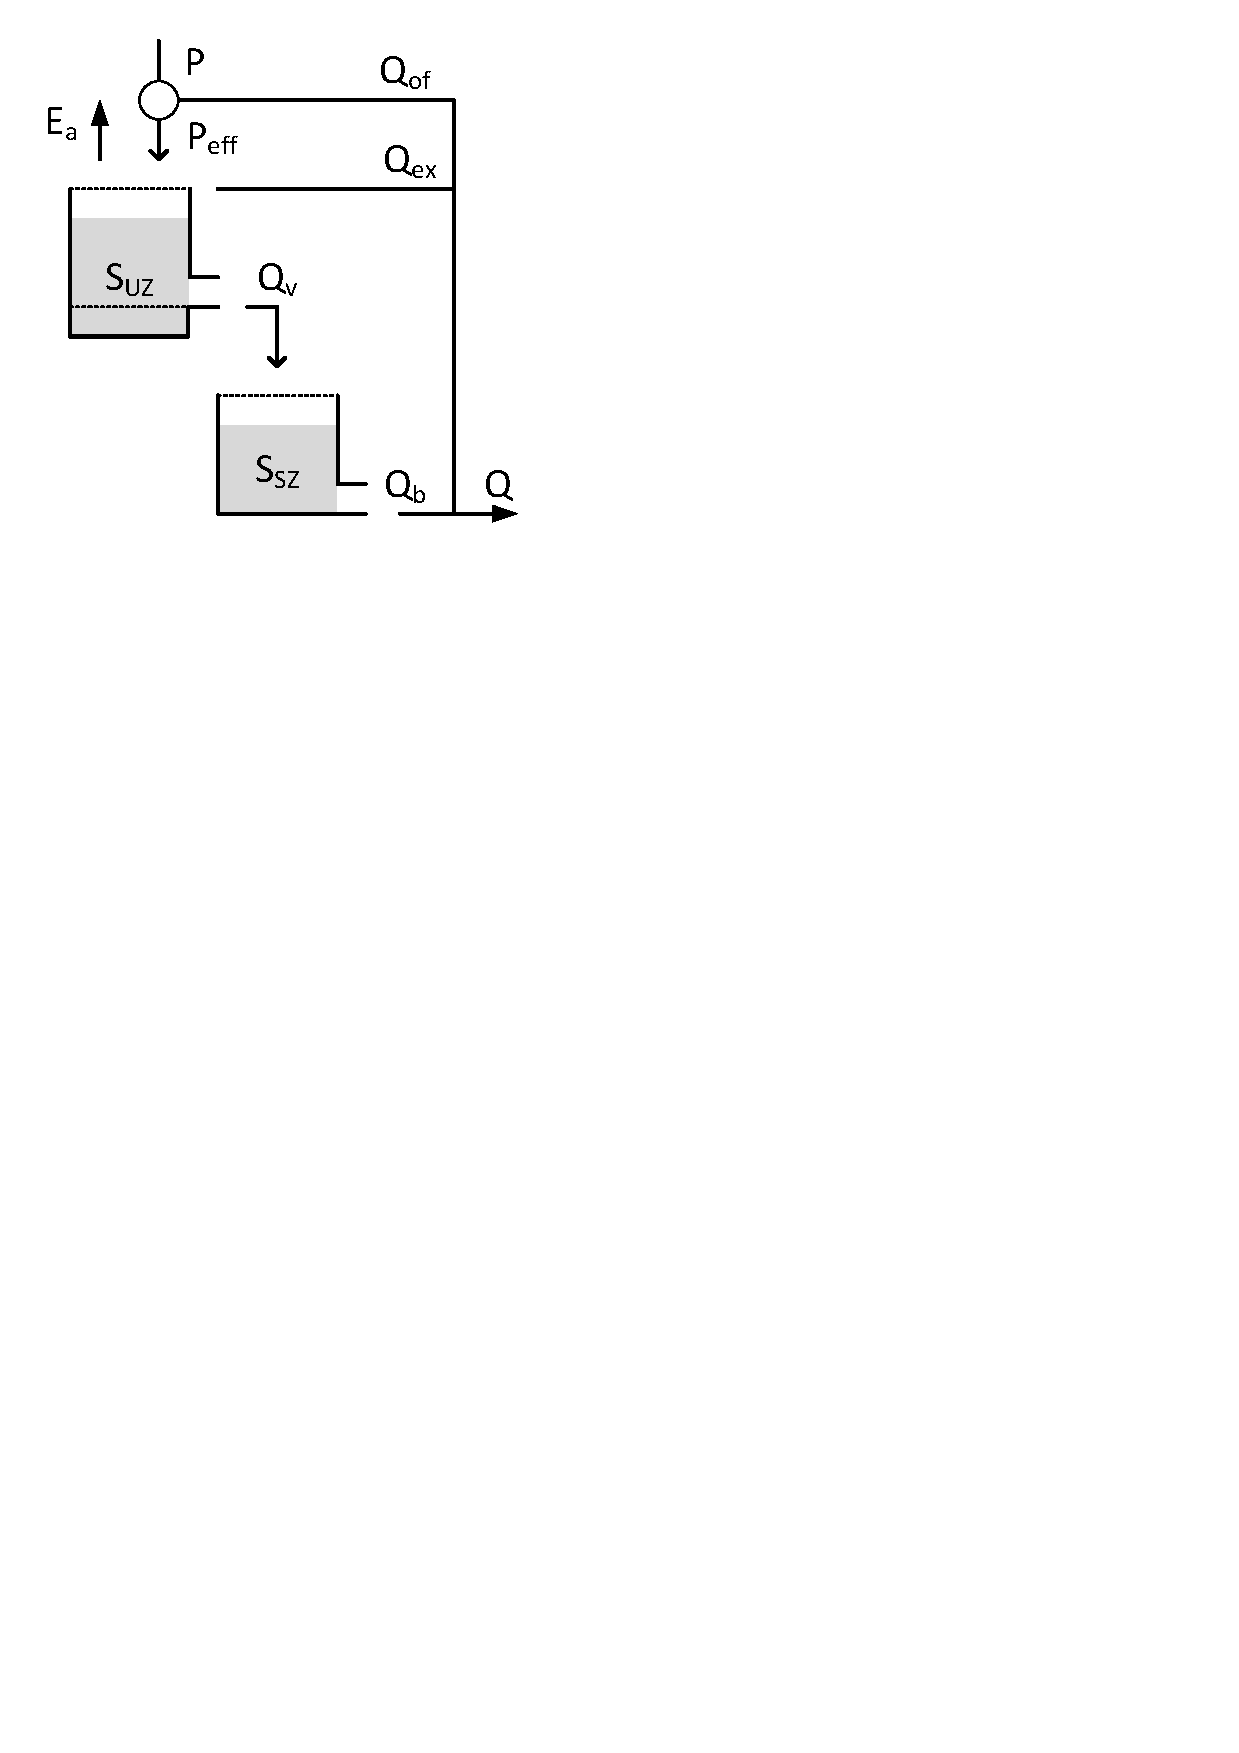
\includegraphics[trim=1cm 21cm 7cm 1cm,width=7cm,keepaspectratio]{./AppA_files/14_schematic.pdf}
\caption{Structure of the TOPMODEL} \label{fig:14_schematic}
\end{wrapfigure}

\begin{align}
	\frac{dS_{UZ}}{dt} &= P_{eff} - Q_{ex} - E_a - Q_v \\
	P_{eff} &= P - Q_{of} = P - A_C*P\\
	Q_{ex} &= \begin{cases}
		P_{eff}, & \text{if } S_{UZ} = S_{uz,max} \\
		0, & \text{otherwise}\\
	\end{cases}\\
	E_a &= 
	\begin{cases}
		E_p, & \text{if } S_{UZ} > S_t*S_{UZ,max} \\
		\frac{S_{UZ}}{S_t*S_{UZ,max}}*E_p, & \text{otherwise}\\
	\end{cases}\\	
	Q_v &=  
		\begin{cases}
		k_d\frac{S_{UZ} - S_t*S_{UZ,max}}{S_{UZ,max}(1-S_t)}, & \text{if } S_{UZ} > S_t*S_{UZ,max} \\
		0, & \text{otherwise}\\
	\end{cases}
\end{align}

} % end of wrapfigure fix
\vspace{0.5cm}

Where $S_{UZ}$ [mm] is the current storage in the combined unsaturated zone and root zone, with $S_t$ [-] (fraction of $S_{UZ,max}$) indicating the boundary between the two and being the threshold above which drainage to the saturated zone can occur. $P_{eff}$ $[mm/d]$ is the fraction of precipitation that does not fall on the saturated area $A_c$ [-], $E_a$ $[mm/d]$ is evaporation that occurs at the potential rate for the unsaturated zone and scaled linearly with storage in the root zone, $Q_{ex}$ $[mm/d]$ is overflow when the bucket reaches maximum capacity $S_{UZ,max}$ [mm], and $Q_v$ $[mm/d]$ is drainage to the saturated zone, depending on time parameter $k_d$ $[d^{-1}]$ and the relative storage in the unsaturated zone compared to the current deficit in the saturated zone.

\begin{align}
	\frac{dS_{SZ}}{dt} &= -Q_v + Q_b\\
	Q_b &= q_0*e^{-f*S_{SZ}}
\end{align}

Where $S_{SZ}$ [mm] is the current storage \emph{deficit} in the saturated zone store, which is increased by baseflow $Q_b$ $[mm/d]$ and decreased by drainage $Q_v$. $Q_b$ relies on saturated flow rate $q_0$ $[mm/d]$, parameter $f$ $[mm^{-1}]$ and current deficit $S_{SZ}$. Total flow:

\begin{align}
	Q &= Q_{of} + Q_{ex} + Q_b\\
	Q_{of} &= A_c*P
\end{align}

The saturated area $A_c$ is calculated as follows. First, the within-catchment distribution of topographic index values is estimated with a shifted 2-parameter gamma distribution \citep{Sivapalan1987,Clark2008a}:

\begin{align}
	f(\zeta) &= \begin{cases}
		\frac{1}{\chi\Gamma(\phi)}\left(\frac{\zeta-\mu}{\chi}\right)^{\phi-1}exp\left(-\frac{\zeta-\mu}{\chi}\right), & \text{if } \zeta > \mu \\
		0, & \text{otherwise}\\
	\end{cases}
\end{align}

Where $\Gamma$ is the gamma function and $\chi$, $\phi$ and $\mu$ are parameters of the gamma distribution. Following \citet{Clark2008a}, $\mu$ is fixed at $\mu=3$ and $\chi$ and $\phi$ are calibration parameters. $\zeta$ represents the topographic index $ln(a/tan\beta)$ with mean value $\lambda = \chi\phi+\mu$. Saturated area $A_c$ is computed as the fraction of the catchment that is above a deficit-dependent critical value $\zeta_{crit}$: 

\begin{align}
	A_c &= \int_{\zeta_{crit}}^{\infty}f(\zeta)d\zeta\\
	\zeta_{crit} &= f*S_{SZ} + \lambda
\end{align}

\newpage
\subsection{Parameter overview}
% Table generated by Excel2LaTeX from sheet 'Sheet1'
\begin{table}[htbp]
  \centering
    \begin{tabular}{lll}
    \toprule
    Parameter & Unit  & Description \\
    \midrule
    $S_{UZ,max}$ & $mm$  & Maximum soil moisture storage \\
    $S_t$ & $-$   & Threshold for drainage as fraction of $S_{UZ,max}$ \\
    $K_d$ & $d^{-1}$ & Runoff coefficient \\
    $q_0$ & $mm~d^{-1}$ & Saturated flow rate \\
    $f$   & $mm^{-1}$ & Shape parameter for connectivity profile \\
    $\chi$ & $-$   & Gamma distribution parameter \\
    $\phi$ & $-$   & Gamma distribution parameter \\
    \bottomrule
    \end{tabular}%
  \label{tab:addlabel}%
\end{table}%

